\section{Implementation and Performance Considerations}
This section is dedicated to discussing some implementation details, as well as some performance aspects of the implementation considering the target hardware. The implementation of GPU device functions has to take into account overheads introduced by uncoalesced memory accesses, maximizing compute throughput, and some other limitations characteristic of the CUDA architecture.

The implementation of the subdivision algorithm and the LoD generation is straightforward, and I did not implement any heavy optimizations because the process only runs once when the scene is loaded, and then the structure is never modified during rendering. This also means that the tree structure can be serialized and written to disk, to facilitate faster loading on subsequent runs. The process could potentially be optimized to run on multiple threads, however, the creation of additional scene primitives implies potentially conflicting writes to the global scene primitive array. There are workarounds to this, like processing subtrees in parallel, and then concatenating their merged primitive vectors, however, this was not the scope of the project, as the overhead can be easily avoided by writing the tree information to disk.

The tree traversal algorithm, however, runs at the beginning of every frame in order to mark the primitives that are eligible for rendering. This means that I have to take special consideration of the performance aspects of the implementation, as overheads that are too large may render this solution ineffective. Because the scene tree is generated in a CPU function call and new nodes are allocated dynamically, we cannot ensure that all the tree data is in a contiguous block of memory after it is generated, as it depends on how the Operating System handles dynamic allocations. After the scene tree is built, I allocate a sufficiently large buffer, traverse the tree, and insert the node information in the buffer, replacing node pointers with buffer indices. This first traversal is also done depth-first, as this is the access pattern when the tree is traversed in the GPU kernel. Now, the tree buffer can be transferred to GPU memory in only one call ensuring memory continuity.

\begin{wrapfigure}{r}{7.5cm}
    \centering
    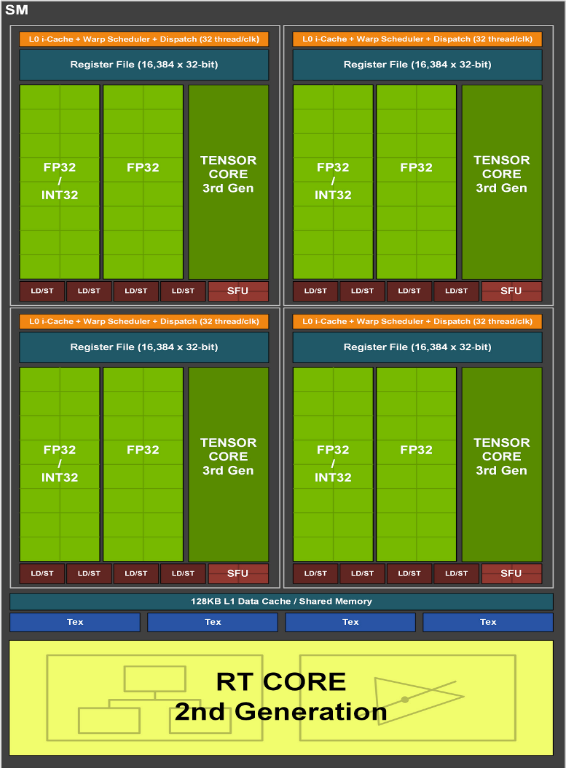
\includegraphics[width=0.7\linewidth]{figures/nvidia_arch.png}
    \caption{NVIDIA GA10x Streaming Multiprocessor architecture \cite{ha107}.}
    \label{fig:nvidia-label}
\end{wrapfigure}

Another significant challenge is the actual tree traversal in the GPU. The CUDA programming model performs well on tasks that perform the same operation on a very large amount of data, and the instructions executed by each thread are mostly the same. Figure \ref{fig:nvidia-label} shows the general architecture of the Streaming Multiprocessor (SM) unit of the NVIDIA Ampere chip architecture. Note that cores inside the SM are grouped into blocks, and all the threads in one block execute the same instructions. This means that a code sequence that diverges in execution can lead to stalls, as some threads wait for others to reach the same execution point. Note that a significant portion of the chip is made up of Tensor Cores, which however cannot be used for this application, as they are mainly designed for performing multiply-add operations on $4\times 4 \times 4$ tensors. This means that we can take advantage only of the standard CUDA cores. Also, the illustration showcases why the INT32 compute throughput is only half of that of FP32.

Traversing a very deep tree poses problems, as threads in a warp will start to diverge in their execution, which leads to stalls. Also, traversing the entire tree from its root node will pose some issues, as the execution is not parallelizable due to the low amount of concurrent data. To address this issue, I am "splitting" the scene tree at the octree leaf nodes. This means that each subtree starting from an octree leaf node will become an independent structure which will be processed in its entirety by one thread. This results in a large set of shallower trees that are completely independent of one another, so they can be traversed in parallel without issues, and the result of the traversal will be the same as a sequential traversal from the scene root. This optimization takes advantage of the fact that the octree component holds no primitive information and is only used for connectivity information, so it can be ignored in the traversal and we can start directly from the BSP roots.

The changes above ensure that the tree can be traversed in parallel by a large number of threads, but I still have to discuss the actual traversal implementation. Tree and graph-like structures in general are notoriously hard to process in GPU kernels, as there is no effective way to ensure coalesced memory accesses and avoid random memory accesses, which come at a great overhead. Moreover, for this application, the computational load is quite small for every node, as we only compute the length of the projected diagonal, and then decide whether to mark the primitive for render or continue the traversal to the children. This means that memory access overheads will be significant and the compute throughput relatively low. Generally, DFS graph traversals are done with recursive function calls, as the implementation is more elegant and CPUs deal well with relatively large function call stacks. The CUDA framework also allows recursivity through its Dynamic Parallelism functionality. However, this is mostly used to launch a computationally-heavy kernel from an already running kernel. In the traversal case, launching multiple kernels recursively will incur a massive amount of launch overhead for a very short computation. Alternatively, the kernel can be used as a wrapper to a device function implementing recursive calls, but in my experiments, this also performed poorly, and extra care has to be taken not to overflow the call stack.

The most efficient DFS implementation I found for this application is to perform the traversal in a loop, using a stack to keep track of the traversed path. Because the trees are quite shallow in the kernel traversal, allocating a stack of 64 elements is enough to ensure there is no overflow, while also being small enough to fit in the local thread memory for fast access. Using the NVIDIA profiling tools, this method showed the lowest percentage of cache misses and the highest compute throughput (even though the value is lower than ideal in order to take full advantage of the architecture).

The scope of this project is to provide an extension to the existing render pipeline without introducing extensive changes. The existing pipeline remains mostly unmodified, and the traversal is done in a separate kernel call before the pre-processing routine. Marking the primitives eligible for render is done through a boolean mask situated in global GPU memory. The scene tree traversal populates the mask with values, then the mask is passed to the pre-processing routine. Then, the pre-processing will quickly discard the primitives that are not marked for rendering in the mask, and the rest of the pipeline remains unchanged.

\paragraph{}
Another optimization I wanted to explore was performing frustum culling during the traversal. This can easily be performed by intersecting the node bounding box with the frustum planes and eliminating nodes that are out of view by terminating their traversal. The performance obtained from this change is quite mixed and heavily depends on what parts of the scene are in view. First of all, even though frustum intersection is trivial to compute, its computational load inside the kernel is quite significant relative to the other operations that are performed, incurring an increasing cost as the traversal goes deeper into the tree. Secondly, primitives that are out of view are removed early in the pipeline by the pre-processing routine by simply projecting the Gaussian centers to the camera plane and using a heuristic to determine if the projected centers are far enough outside the image plane to be discarded. 

On camera positions that contained the most detailed parts of the scene in view, culling in the traversal did not bring any improvements, and in some cases even incurred a small overhead. The only situation when it is beneficial is when complex parts of the scene are outside the frustum, so many nodes and primitives can be removed early from the traversal by culling large nodes close to the root. Performance metrics and examples of this are discussed in the Results chapter. 